%%
%% This is file `mcmthesis-demo.tex',
%% generated with the docstrip utility.
%%
%% The original source files were:
%%
%% mcmthesis.dtx  (with options: `demo')
%% 
%% -----------------------------------
%% 
%% This is a generated file.
%% 
%% Copyright 
%%     2010 -- 2015 by Zhaoli Wang
%%     2014 -- 2016 by Liam Huang
%% 
%% This work may be distributed and/or modified under the
%% conditions of the LaTeX Project Public License, either version 1.3
%% of this license or (at your option) any later version.
%% The latest version of this license is in
%%   http://www.latex-project.org/lppl.txt
%% and version 1.3 or later is part of all distributions of LaTeX
%% version 2005/12/01 or later.
%% 
%% This work has the LPPL maintenance status `maintained'.
%% 
%% The Current Maintainer of this work is Liam Huang
%% 
\documentclass{mcmthesis}
\mcmsetup{CTeX = false,   % 使用 CTeX 套装时,设置为 true
        tcn = 86483, problem = E,
        sheet = true, titleinsheet = true, keywordsinsheet = true,
        titlepage = false, abstract = true}
\usepackage{palatino}
\usepackage{booktabs}
\usepackage{lipsum}
\usepackage{wrapfig}
\usepackage{geometry}
% 这两行可以让点击图片引用显示整个图片,而不是只有字
\usepackage{caption}
\captionsetup{hypcap=true}

\title{The \LaTeX{} Template for MCM Version \MCMversion}
\author{\small \href{http://www.latexstudio.net/}
  {\includegraphics[width=7cm]{mcmthesis-logo}}}
\date{\today}

\renewcommand\arraystretch{1.5}
\newcolumntype{I}{!{\vrule width 1.2pt}}
\newlength\savedwidth
\newcommand\whline{\noalign{\global\savedwidth\arrayrulewidth
                            \global\arrayrulewidth 3pt}%
                   \hline
                   \noalign{\global\arrayrulewidth\savedwidth}}
\newlength\savewidth
\newcommand\shline{\noalign{\global\savewidth\arrayrulewidth
                            \global\arrayrulewidth 1.5pt}%
                   \hline
                   \noalign{\global\arrayrulewidth\savewidth}}


% \geometry{left=2.0cm,right=2.0cm,top=2.5cm,bottom=2.5cm}
\geometry{top=2.5cm,bottom=2.5cm}
% 以上导言区
\begin{document}
\begin{abstract}
\lipsum[1]
\begin{keywords}
keyword1; keyword2
\end{keywords}
\end{abstract}
\maketitle
\tableofcontents
% \newpage

% \lipsum[2]
% \begin{itemize}
% \item minimizes the discomfort to the hands, or
% \item maximizes the outgoing velocity of the ball.
% \end{itemize}
% We focus exclusively on the second definition.

% \begin{itemize}
% \item the initial velocity and rotation of the ball,
% \item the initial velocity and rotation of the bat,
% \item the relative position and orientation of the bat and ball, and
% \item the force over time that the hitter hands applies on the handle.
% \end{itemize}
% \lipsum[3]
% \begin{itemize}
% \item the angular velocity of the bat,
% \item the velocity of the ball, and
% \item the position of impact along the bat.
% \end{itemize}
% \lipsum[4]
% \emph{center of percussion} [Brody 1986], \lipsum[5]

% \begin{Theorem} \label{thm:latex}
% \LaTeX
% \end{Theorem}
% \begin{Lemma} \label{thm:tex}
% \TeX .
% \end{Lemma}
% \begin{proof}
% The proof of theorem.
% \end{proof}
\newpage
\section{Introduction}
\subsection{Background}
Climate is the most important environmental condition for human activities.
Climate change has had a negative impact on the ecological environment in 
many countries and regions. It is estimated that if the coastal population 
increases and the sea level rises by 40 cm, the number of people affected by 
flood disasters will increase by 75 million to 206 million each year, 90\% of
which are in Africa and Asia. Poor people's ability to adapt to climate change 
are limited by livelihood assets and livelihood pressure. High frequency of
extreme weather events will reduce the recovery time of poverty population, 
and keep them in a fragile state for a long time. Some underdeveloped 
countries not only have to deal with the risks posed by climate change, 
but also have to deal with the impact of economic globalization, 
and are more vulnerable to failure.This phenomenon is called vulnerability.\\\\
In recent years, many international organizations have conducted vulnerability 
assessments in developing countries. The United States Agency for International
Development (USAID) famine warning system focuses on the vulnerability of 
food security in African regions.The Vulnerability Assessment committee(VAC) 
evaluated the comprehensive vulnerability of six African countries food safety 
and living condition. The Department for International Development (DFID)
focuses on rural sustainable Development and poverty alleviation in developing
countries. Vulnerability assessment is helpful for scientists and 
policymakers to understand the influence of environmental changes, 
to explore potential factors hinder the social effective response, 
to understand the vulnerable population distribution and the causes 
of vulnerability, and find out the ways to reduce vulnerability and 
increase the adaptability.\\\\
At present, many studies devote to evaluate natural ecosystem vulnerability, 
and has built many widely used quantitative methods,to figure out the 
vulnerability level and distribution of the natural ecological system, 
to predict the adaptation of natural ecosystems to risk in the future.However, 
scientists, policymakers, and ngos tend to focus more on regional 
vulnerability assessments, in order to connect with decisions. Different 
from the natural ecosystem, region is a natural-economic-social complex 
system, so the fragility of the natural ecosystem does not necessarily lead 
to a vulnerable. Human suffer from environmental impact and risk, such as 
natural disasters and limited resources, meanwhile,they adapt and transform 
the natural environment, using natural material and energy to develop itself.
Due to the complexity of the system in the region, it is difficult to 
quantitatively assess its vulnerability thus causing a gap in widely-used 
quantitative method.In the context of climate change, the situation in some
less-developed regions of the world will be severely affected, so it is 
particularly urgent to identify vulnerable areas and take measures to 
address them.


\subsection{Restatement of the Problem}
A fragile state inherently exists vulnerability of natural conditions 
like natural disasters, the decrease of the cultivated land, unpredictable 
weather and rising temperature.coupled with the turbulent political situation, 
backward economic development, poor sanitation, the condition will get worse. 
Therefore, when considering the impact of climate on national vulnerability, 
it is not possible to consider only one single factor of climate, but also to
consider the joint role of economic, political and social factors.\\\\
However, various aspects, including climate pressure will not necessarily 
make a country vulnerable. If a country has a strong government and a high 
level of economy, the country will have a strong ability to adapt to respond
to climate change. As a result, countries are less vulnerable to climate 
change. It appears that the vulnerability of a country is not only affected
by external pressure, but more depends on the country's ability to fight 
against external pressure. In the process of modeling, we must give full 
consideration to country's ability to resist pressure and adapt.
\subsection{Our Work}
  \textbf{Work\_1, clear the definition of vulnerability and research object:} We 
  define vulnerability as the degree to which the system is susceptible to adverse effects 
  and lack of the ability to cope with adverse effects. We also define that vulnerability 
  is a function of sensitivity and adaptability. We will explain these two concepts 
  (sensitivity and adaptability) below.\\ We regard the overall vulnerability of 
  countries as a \textbf{natural-economic-social composite system} under the influence of 
  multiple factors. The vulnerability of the country is related to the country's 
  climate sensitivity index, economic development status, social stability and 
  other factors.\\\\
  \textbf{Work\_2, collect data on factors affecting national vulnerability:} The data we
  collect include sensitivity data (Extreme weather、Average precipitation in depth、Climate
  sensitivity index、Food security index、National risk index、Health index、mortality、
  Crime index、global firepower index, hunger index,  proportion of agricultural output 
  in GDP, ethnic diversity and refugee Numbers) and adaptability data(GDP per capita, 
  Poeple's Fredom index, Government Effectiveness index, Political Stability index).\\\\
  \textbf{Work\_3, calculate the correlation between climate and other factors:} we 
  calculate the relevance of various factors about economic, political, social 
  and climatic that can affect the vulnerability of the country, then choose 
  factors that are clearly relevant to climate,and \textbf{explain why and how the 
  climate affects these facts}.




\section{Analysis of Problem}

\section{General Assumptions and Data Analysis}
\subsection{General Assumptions}
\begin{itemize}
  \item We ignore the effects of individual factors on the model caused by year inconsistency.
  \item We assume that the overall vulnerability of the country is only determined by national sensitivity and adaptability.
  \item We assume that countries sensitivity index is determined only by extreme weather、average precipitation in depth、climate sensitivity index、food security index、national risk index、health index、mortality、arime index、global firepower index, hunger index,  proportion of agricultural output in GDP, ethnic diversity and refugee Numbers.
  \item We assume that national adaptability is determined only by GDP per capita, Poeple's Fredom index, Government Effectiveness index, Political Stability index.
  \item We assume that the factors other are independent and non-interference, but climate is not included.
  \item We assume that vulnerability can be effectively quantified by the above data.
  \item We assume that the data we collect is true and valid.
\end{itemize}
\subsection{Data Analysis}
% 表格
% \begin{table}[]
%   \centering
%   \caption{My caption}
%   \label{my-label}
%   \setlength{\tabcolsep}{7mm}{
%   \begin{tabular}{l|l|l|l|l|l|l|l|l|l|l|l}
%   \shline
%   \multicolumn{2}{lI}{\textbf{asasd}} & \multicolumn{10}{l}{\textbf{ssssssssssssssssssssss}} \\ \hline
%   \multicolumn{2}{lI}{dddd}           & \multicolumn{10}{l}{ddddddddddddddddddddd}           \\ \hline
%   \multicolumn{2}{lI}{}               & \multicolumn{10}{l}{}                                \\ \hline
%   \multicolumn{2}{lI}{}               & \multicolumn{10}{l}{}                                \\ \hline
%   \multicolumn{2}{lI}{}               & \multicolumn{10}{l}{}                                \\ \hline
%   \multicolumn{2}{lI}{}               & \multicolumn{10}{l}{}                                \\ \hline
%   \multicolumn{2}{lI}{}               & \multicolumn{10}{l}{}                                \\ \hline
%   \multicolumn{2}{lI}{}               & \multicolumn{10}{l}{}                                \\ \hline
%   \multicolumn{2}{lI}{}               & \multicolumn{10}{l}{}                                \\ \shline
%   \end{tabular}}
%   \end{table}  

\section{Variable Description and Research Method}
\subsection{Variable Description}
\subsection{Research Method}
% 插图
% \begin{figure}[h]
% \small
% \centering
% 
\includegraphics[width=12cm]{test1.jpg}
% \caption{asssssa} \label{fig:aa}
% \end{figure}

% 引用
% \eqref{aa}
% \begin{equation}
% a^2 \label{aa}
% \end{equation}

% 公式
% \[
%   \frac{\mathrm{d} C_{1}}{\mathrm{d} t}= \left 
%   ( 1-\frac{C}{R} \right )^{P_{I}}\frac{\mathrm{d} I}
%   {\mathrm{d} t}\frac{C_{I}}{I} \eqno (3)
% \]




\section{Fragile State Neural Network Model}
The study of national vulnerability indicators requires strong professional
background knowledge, but we can't derive the relationship between climate
and vulnerability through an intuitive approach from the data given in the 
problem. So, through collecting data, by using the strong self-organization, 
self-adaptive and self-learning ability of neural network, the nonlinear 
mapping of independent variables and national fragility can be completed 
without fully understanding the relationship among climate, politics, 
economy and national fragility. Combined with the above considerations, 
We established a neural network to derive a national vulnerability model 
including climatic factors.
\subsection{Model building}
\subsubsection{Introduction to the principle of BP neural network}
BP Neural Network is a kind of multi-layer feedforward neural network, 
which is mainly characterized by forward transmission and deviation back 
propagation.In forward transmission, the input signal is processed from 
the input layer through the hidden layer to the output layer.The state of 
each layer of neurons affects only the next layer of neurons.If the output 
layer does not get the desired output, it is transferred to the reverse 
propagation, and the network weight and threshold are adjusted according 
to the predicted error, so that the BP neural network prediction output 
is constantly approaching the expected output. A simple BP Neural Network 
is like Figure \ref{fig:nn} as follow.
\begin{figure}[h]
\small
\centering
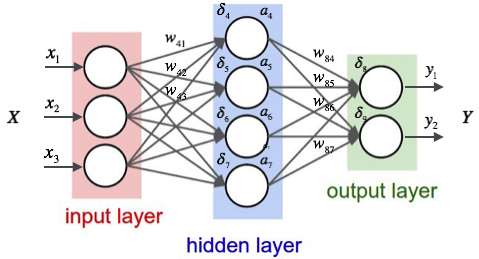
\includegraphics[width=10cm]{neuralNetwork.png}
\caption{Neural Network} \label{fig:nn}
\end{figure}

\section{Model Testing}

\section{Sensitivity Analysis}
\subsection{Impact of x}
\subsection{Impact of y}

\section{Strengths and Weaknesses}
\subsection{Strengths of Models}
\subsubsection{Inclusive}
\subsubsection{Quantification}
\subsubsection{Simple but Universal}
\subsubsection{Visible and Understandable}
\subsection{Weaknesses of Models}
\subsubsection{Accuracy Relies on Statistics}
\subsubsection{Xxx Is Not Included}
% 图文混排
% \begin{wrapfigure}{l}{4.5cm}%靠文字内容的左侧
%   
\includegraphics[width=4cm]{test1.jpg}\\
%   \caption{Podala Palace, Tibet}\label{fig:tibet}
%   \end{wrapfigure}

To begin with, we searched a large number of papers that discuss the spread of
Ebola to help us deepen the understanding of the problem. Chowell et al. provided a
large amount of background information and their work [6] served as an important
introduction. We found that a few of the papers used the traditional epidemic model to
predict the transmission of the disease such as the SEIR model used by Althaus [11] to
estimate the reproduction number of the virus\cite{bib1,bib2} during the 2014 outbreak. Therefore, we
also applied the SEIR model in the early stage to predict the spread of Ebola. Later, we
found out that the Ebola virus has some specific feathers that also needed to be
considered and that are, the potential transmission threat posed by the highly infectious
corpses, the improved infection control and reduced transmission rate if patients can be
treated in hospitals, and the powerful intervention method: contact tracing. After taking
all these critical factors into consideration, we improved our original epidemic model.

% 论文引用
\begin{thebibliography}{99}
\bibitem{bib1} D.~E. KNUTH   The \TeX{}book  the American
Mathematical Society and Addison-Wesley
Publishing Company , 1984-1986.
\bibitem{bib2}Lamport, Leslie,  \LaTeX{}: `` A Document Preparation System '',
Addison-Wesley Publishing Company, 1986.
\bibitem{bib3}\url{http://www.latexstudio.net/}
\bibitem{bib4}\url{http://www.chinatex.org/}
\end{thebibliography}

% 附录
\begin{appendices}

\section{First appendix}

\lipsum[13]

Here are simulation programmes we used in our model as follow.\\

\textbf{\textcolor[rgb]{0.98,0.00,0.00}{Input matlab source:}}
\lstinputlisting[language=Matlab]{./code/mcmthesis-matlab1.m}

\section{Second appendix}

some more text \textcolor[rgb]{0.98,0.00,0.00}{\textbf{Input C++ source:}}
\lstinputlisting[language=C++]{./code/mcmthesis-sudoku.cpp}

\end{appendices}
\end{document}

%% 
%% This work consists of these files mcmthesis.dtx,
%%                                   figures/ and
%%                                   code/,
%% and the derived files             mcmthesis.cls,
%%                                   mcmthesis-demo.tex,
%%                                   README,
%%                                   LICENSE,
%%                                   mcmthesis.pdf and
%%                                   mcmthesis-demo.pdf.
%%
%% End of file `mcmthesis-demo.tex'.
